\documentclass[oneside, final, 14pt]{extarticle}
% rewrite with extreport
\usepackage[utf8]{inputenc}
\usepackage[russianb]{babel}
\usepackage[paper=a4paper, left=3cm, top=2cm, bottom=2cm, right=1cm]{geometry}
\usepackage{indentfirst}
\usepackage{amsmath}
\usepackage{amssymb}
\usepackage{verbatim}
\usepackage{ntheorem}
\usepackage{graphicx}
\usepackage{multicol}
\usepackage{moreverb}
\usepackage{listings}

\begin{document}

\begin{titlepage}

%\newgeometry{margin=1cm}

\centerline{\bf МИНИСТЕРСТВО ОБРАЗОВАНИЯ РЕСПУБЛИКИ БЕЛАРУСЬ}
\bigskip
\bigskip
\centerline{\bf БЕЛОРУССКИЙ ГОСУДАРСТВЕННЫЙ УНИВЕРСИТЕТ}
\bigskip
\bigskip
\centerline{\bf ФАКУЛЬТЕТ ПРИКЛАДНОЙ МАТЕМАТИКИ И ИНФОРМАТИКИ}
\bigskip
\bigskip
\centerline{\bf Компьютерная Безопасность Распределенных Систем}
\vfill
\vfill
\vfill
\begin{centering}
  {\bf СИНЯК СЕРГЕЙ АЛЕКСАНДРОВИЧ \\
       СИНЯК ВИКТОР АЛЕКСАНДРОВИЧ \\}
\end{centering}
\bigskip
\bigskip
\begin{centering}
  {\bf СИМУЛЯЦИЯ MITM АТАКИ \\
       в PEAP ПОСРЕДСТВОМ HOSTAP \\}
\end{centering}
\vfill
\begin{centering}
  {
  Учебный Проект \\
  студентов 4 курса, 3 группы, специальность <<информатика>> \\}
\end{centering}
\vfill
\vfill
\hfill
\begin{minipage}{0.35\textwidth}
  {\bf Преподаватель \\
  {\small{\it Галибус Татьяна \\ Васильевна}}}
\end{minipage}
\vfill
\vfill
\centerline{\large \bf Минск, 2016}

\restoregeometry

\end{titlepage}

\setcounter{page}{2}

\tableofcontents

\cleardoublepage

\section{Введение}

Мы бы хотели продемонстрировать анализ PEAP,
с последующей реализацией MITM эксплоита.
Суть заключается в симуляции атаки.
В качестве отправной точки была принята публикация
\cite{tap2002},
датированая 2002 г., полученая и опубликованая в 2013 г.
Там мы наблюдаем исследование туннелированных протоколов
аутентификации.
Подавляющее большинство унаследованных, а следовательно
широко распостраненных протоколов
требуют обновления, дабы соотвествовать последним
стандартам безопасности.
При этом сильно важно сохранить унаследованный код
и инфаструктуру.
Если протокол подвержен проблемам слабого пароля
или не скрывает личность пользователя,
то он может быть протуннелирован некоторым внешним протоколом.
В этом случае, сервер сетевого доступа
аутентифицируется для клиента внешним протоколом,
а затем клиент аутентифицируется для сервера внутренним
(предпологаемо унаследованным).
Как только протокол завершен, обе стороны завершают коммуникацию
генерацией токенов,
в случае успешной аутентификации.
Если мы говорим о зашифрованном сетевом доступе,
то результирующие токены есть сессионные ключи,
которые определяют шифрование дальнейших сообщений
передача которых произойдет посредством
канал связи, который и был аутентифицирован.

\cleardoublepage

\section{Криптобиндинг}
Внутренний протокол должен бы криптографически связан
с внешним.
Работа \cite{tap2002} упоминает два пути:
\begin{enumerate}
  \item неявный способ, то есть результирующий ключ $K$ получен
    путём односторонней хэш функции, которая затрагивает как секретные
    данный внешнего протокола $T$,
    там и секретный ключ $S$ из внутреннего протокола.
  \item явное криптографическое связывание, это когда
    особенное значение проверки $V$
    сгенерировано тем же способом из $T$ и $S$,
    и проверено некоторой аутентифицирующей сущностью
    на равенство между сторонами.
\end{enumerate}

Для снижение наложенных правок в унаследованном протоколе,
все эти соображения следует принять в рассмотрение
на уровне внешнего протокола.

Это очень важно добавить криптографическое связывание,
потому что в противном случае внутренний протокол
аутентификации применяется будучи не сведомым о том,
существует ли защищающий туннель или нет.
Такая криптографическая схема является уязвимой к атаке
человек-по-середине.

\cleardoublepage

\section{PEAP с MSCHAPv2}

Давайте рассмотрим PEAP с MSCHAPv2, что часто используется
в Wi-Fi сетях для аутентификации клиентов.
Главная схема имеется название WPA-Enterprise,
и воплошает обычный WPA/WPA2 стандарт зашифрованной беспроводной коммуникации.
Принципиальное различие в аутентификации и выводе сессионных ключей.
В то время как обычный WPA/WPA2 стандарт полагается на одну парольную фразу,
которая известна всем пользователям беспроводной точки,
Enterprise версия разрешает полноценную аутентификацию посредством
EAP автомата.
Это концепт аутентификации общего назначения для разнообразной коллекции
унаследованных, широко распостраненных схем.
Например, вы можете задействовать Базу пользователей Windows Server'а
настроив сервер сетевого доступа на протокол PEAP с MSCHAPv2
который будет подключаться через RADIUS протокол к серверу пользователей
и аутентифицировать
клинета внутри защищенного TLS туннеля через MSCHAPv2 схему.
В начале клиент, аутентифицирует NAS путём проверки сетевого сертификата,
это происходит в течение протокола TLS Handshake.
Сервер, будучи успешно аутентифицирован и аувторизирован, даёт начало
инициализации обеими сторонами TLS туннеля,
через генерацию общего главенствующего ключа TLS.
TLS схема дозволяет создание общих секретов для обоих сторон,
и является защищенной против атак рода человек-по-середине,
если только пользователь или серевер не пропускают проверку сертификата.
Это стоит того, чтобы отметить, а именно, многие платформы
позволяют тем или иным путём, игнорировать проверку сетевого сертификата сервера,
оставляя пользователей незащищенными.
Практика такого бездумного поведения исходит от использование
самоподписанных сертификатов для аутентификации и работы TLS.
И если соотвествующие уполномоченные не беспокояться о предоставлении
сертификата пользователям
и иногда даже стимулируют опускание проверки,
пользователи, в этом случае, обычно стоят перед выбором
использовать небезопасную сеть,
или отказаться от её ресурсов.
Некоторые замятет, что мы можем применить фиксирование сертификата,
что немного более безопасно, чем не проверять его вовсе.
Да, мы действительно можем это.

\cleardoublepage

\section{Анализ инструментов}

Исходная цель была следующей:
Так если я есть тот самый пользователь который пропускает проверку сертификата,
и есть использует ту самую конфигурацию -- PEAP с MSCHAPv2.
То почему бы не использовать других, ничего не подозревающих пользователей,
путём написания реального эксплоита.

Среди доступных средств, проект hostap \cite{hostap-w1fi}
выступал впереди,
потому что это реализация как клиента так и сервера
для схем шифрования беспроводных сетей.
Кодовая база является регулярно поддерживаемой,
широко распостраненной,
фактически все Android телефоны, и наверняка почти каждая
linux машина используют wpa\_supplicant, это клиентское приложение
для аутентификации и генерации сессионных ключей в Wi-Fi сетях.
Приложение hostapd представляет собой дополнение для серверной стороны
по отношению к wpa\_supplicant.
Архитектура приложения является модульной, и содержит реализации
EAP автоматов для клиента и сервера.
Даже более, там есть работающий пример, который симулирует
общение двух EAP автоматов -- клиента и сервера.
Настроенный протокол в точности PEAP с MSCHAPv2.

Мы можем врядли указать какие-либо серъёзные недостатки данного подхода.
Хотя некоторые факты стоит упомянуть.
Уже существует публикация датированная 2008 годом,
с конференции по безопасности SHMOOCON 2008 \cite{whfs-peap-shmoocon-2008}.
Двое ребят рассказывали о создание мнимого сервера для реальных клиентов,
но их атака базируется на собирании сообщений жертв
в рамках протокола MSCHAPv2,
затем клиенты уведомляются об успешной аутентификации.
Те сообщения позволяет быстрые атаки по словарю на пароли.
В работе также представлена пропатченная версия hostapd (hostapd-wpe \cite{hostapd-wpe})
которая реализует их эксплоит.
Сервер собирает специальные хэшы,
которые затем взламываются утилитой выступающих,
по имени asleap.
Хотя, эта работа явно перекликается с нашей,
атаке предоставленная в ней отличается от рассматриваемой
здесь.
Они взламывают слабость парольных хэшей в MSCHAPv2,
а мы собираемся пробрасывать полносью всё общение протокола
и не заинтересиваны в его содержимом.
Таким образом, вы видите, что hostap был уже использован для схожих целей.
Мы не сведомы о скорости взлома пароля,
но полагаем, что это отнимет больше времени, чем просто проброс сообщений
между клиентом и сервером через узел человека-по-серидине.

\cleardoublepage

\section{Симуляция атаки человек-по-середине и её код}

Код \cite{GMI}  который мы предоставляем, симулирует атаку,
и не является реальным эксплоитом.

Прямолинейная реализация есть в работе \cite{tap2002},
и имеет следующий вид:
\begin{enumerate}
  \item Человек-по-середине ждем законное устройство до момента его входа
    в не тунеллированный унаследованный протокол удалённой аутентификации
    и захватывает первоначальное сообщение посланное законным клиентом.
  \item Человек-по-середине инициализирует туннелированный протокол аутентификации
    с аутентифицирующим агентом.
  \item После того, как туннель установлен между человеком-по-середине и аутентифицирующим
    агентом, MitM начинает проброс сообщение аутентификации от законного клиента
    через туннель.
  \item MitM разворачивает сообщение унаследованного протокола полученные через туннель
    от аутентифицирующего агента
    и пробрасывает их к законному клиенту.
  \item После того, как удалённая аутентификации закончилась успешно,
    MitM создает сессонные ключи на основе тех же самых ключей,
    что были использовны для TLS туннеля.
\end{enumerate}

Исходный eap\_example был расширен и содержит 4 EAP автомата,
а именно Клиент Боба, Сервер Алисы, Клиент Евы и Сервер Евы.
Здесь, Боб играет роль жертвы,
и Алиса есть законный сервер.
Автоматы Клиента и Сервера Евы представляют
человека-по-середине,
где очевидно,
что Клиент Боба общается с Сервером Евы,
и Сервер Алисы аутентифицирует Клиента Евы.

В реальной жизни, MitM может вклиниться путем предоставления
точки доступа со схожей <<внешностью>> но которая имеет
более мощный сигнал чем законная.
Если сеть не использует шифрования,
то самый быстрый путь для применение MitM атаки это включить мобильный
интернет на вашем Android телефоне,
затем создать точку доступа с тем же самым имененм, что и точка доступа
под атакой.
После, вам нужно подойте близк к жертве.
В интернете, вы можете наткнуться на пакет aircrack-ng,
который позволяет послать направленный пакет деатентификации,
там, чтобы приложение клиента было вынуждена создать сессию
занаво,
и с большой вероятностью, ваш телефон будет выбран как сервер доступа к сети.

Но такая схема не работает для шифрованного сетевого общения,
если только вы не знаете пароля для подделывания личности сервера,
или любого другого требуемого секрета для корректной аутентификации.

В нашем случае, то есть с WPA-Enterprise точкой достуа,
настроенной на PEAP с MSCHAPv2,
MitM может быть применен,
но мобильный интернет не сработает,
поскольку аутентификации происходит у реального сервер досутпа к сети,
который мы не моожем симулировать. Мы не знаем пароля жертвы.

Мы можем подделать личность NAS втечение протокола TLS Handshake.
Потому что единственное доказательство личности сервер
есть сетевой сертификат,
предположительно само-подписанный или обеспеченный цепью
в направлении доверенного CA. Но если клиент, не проверяет это,
и опция доступна повсеместно,
то MitM атака тривиальна.
Всё что нам нужно это принять участие в диалоге TLS Handshake.

Это первая фаза в PEAP. После, на сцену выходит протокол MSCHAPv2.
Он туннелирован через TLS протокол.

На рисунках 1, 2 и 3 вы можете увидеть обычную сессию PEAP,
общий вид сессии атаки человек-по-середине в PEAP
и детальную проброску MSCHAPv2.

\begin{figure}
  \centering 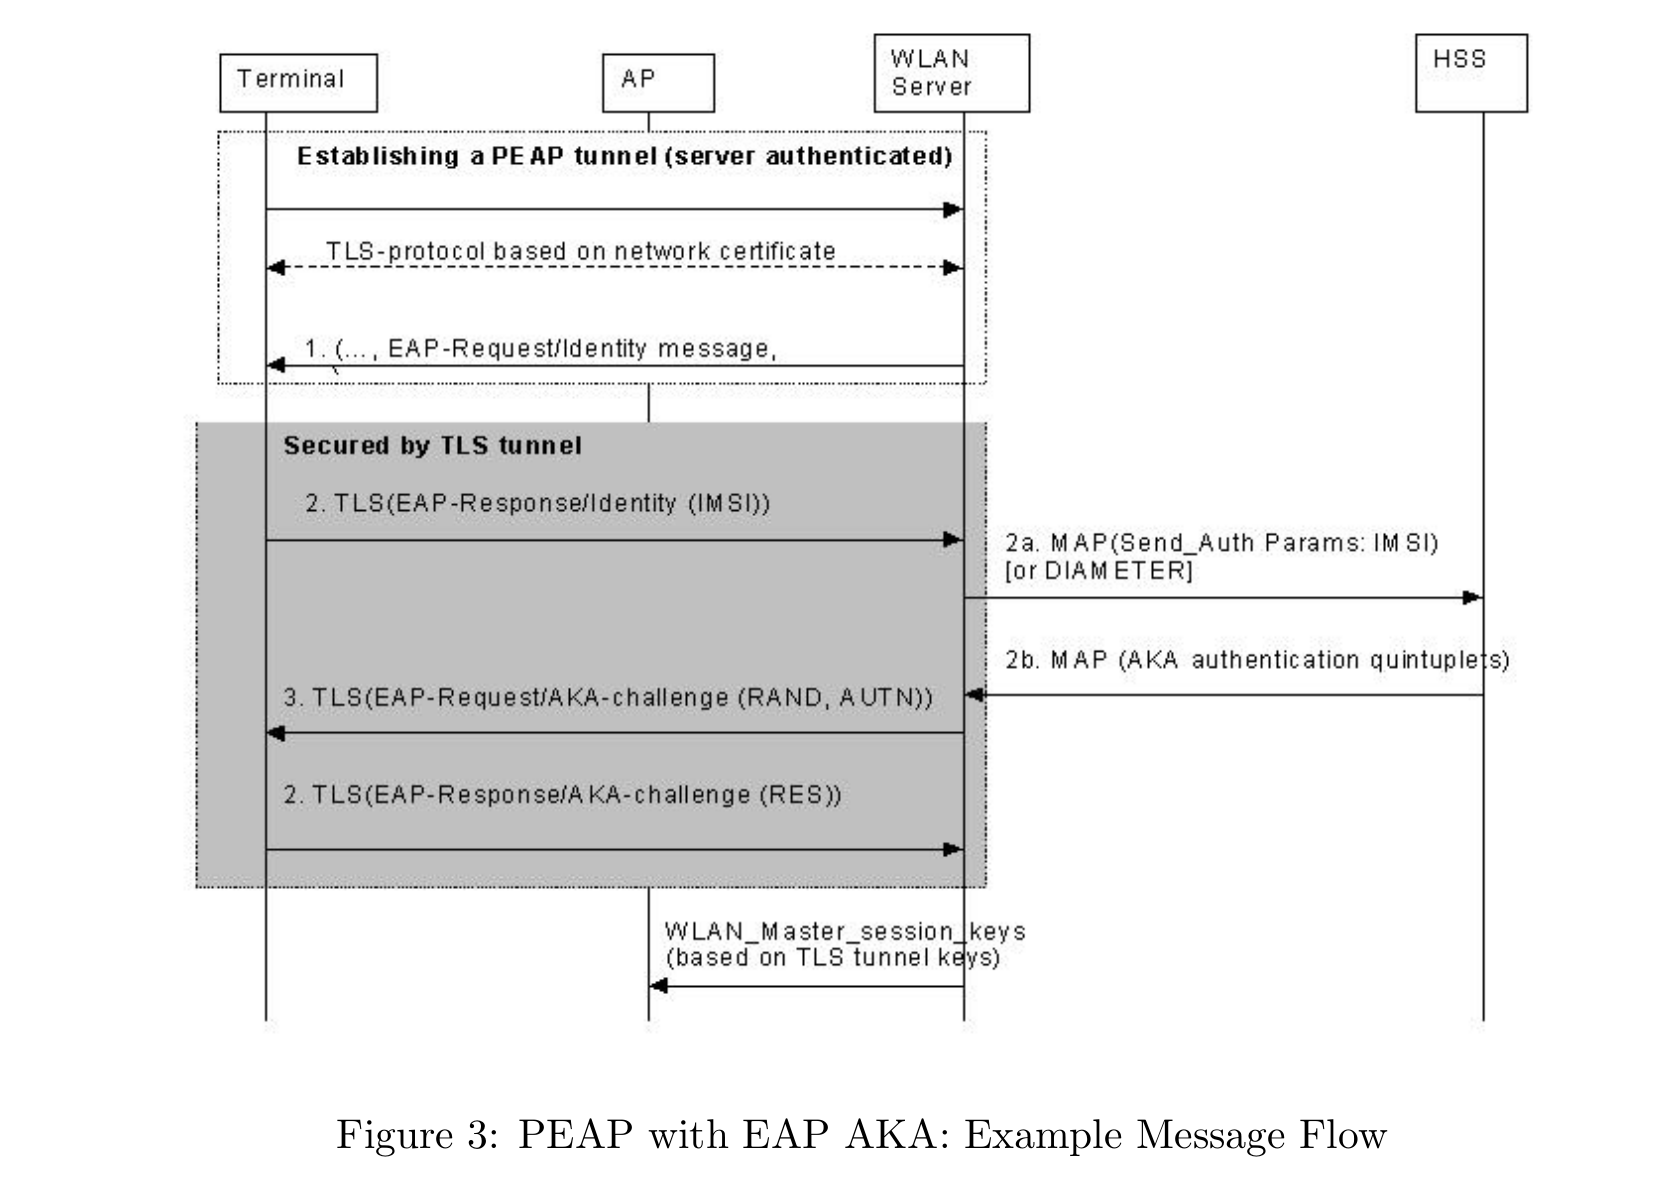
\includegraphics{res/peap-session-fig.png}
  \caption{Обычная сессия PEAP}
\end{figure}

\begin{figure}
  \centering 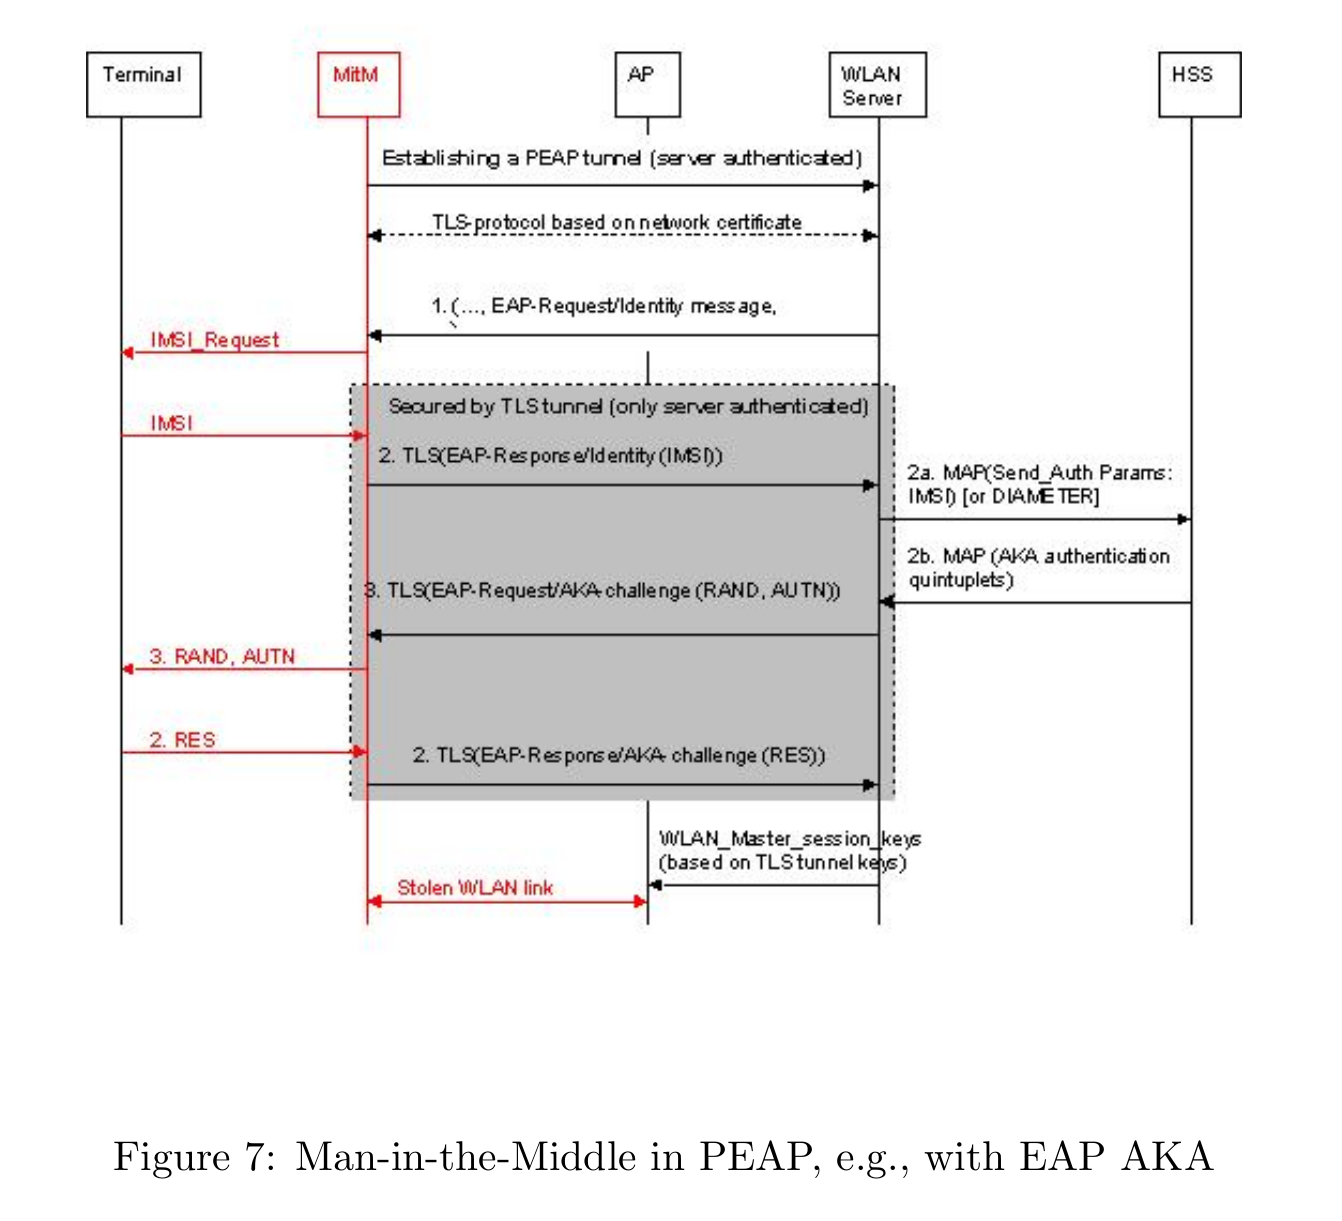
\includegraphics{res/peap-mitm-general.png}
  \caption{Общий вид сессии атаки человек-по-середине в PEAP}
\end{figure}

\begin{figure}
  \centering 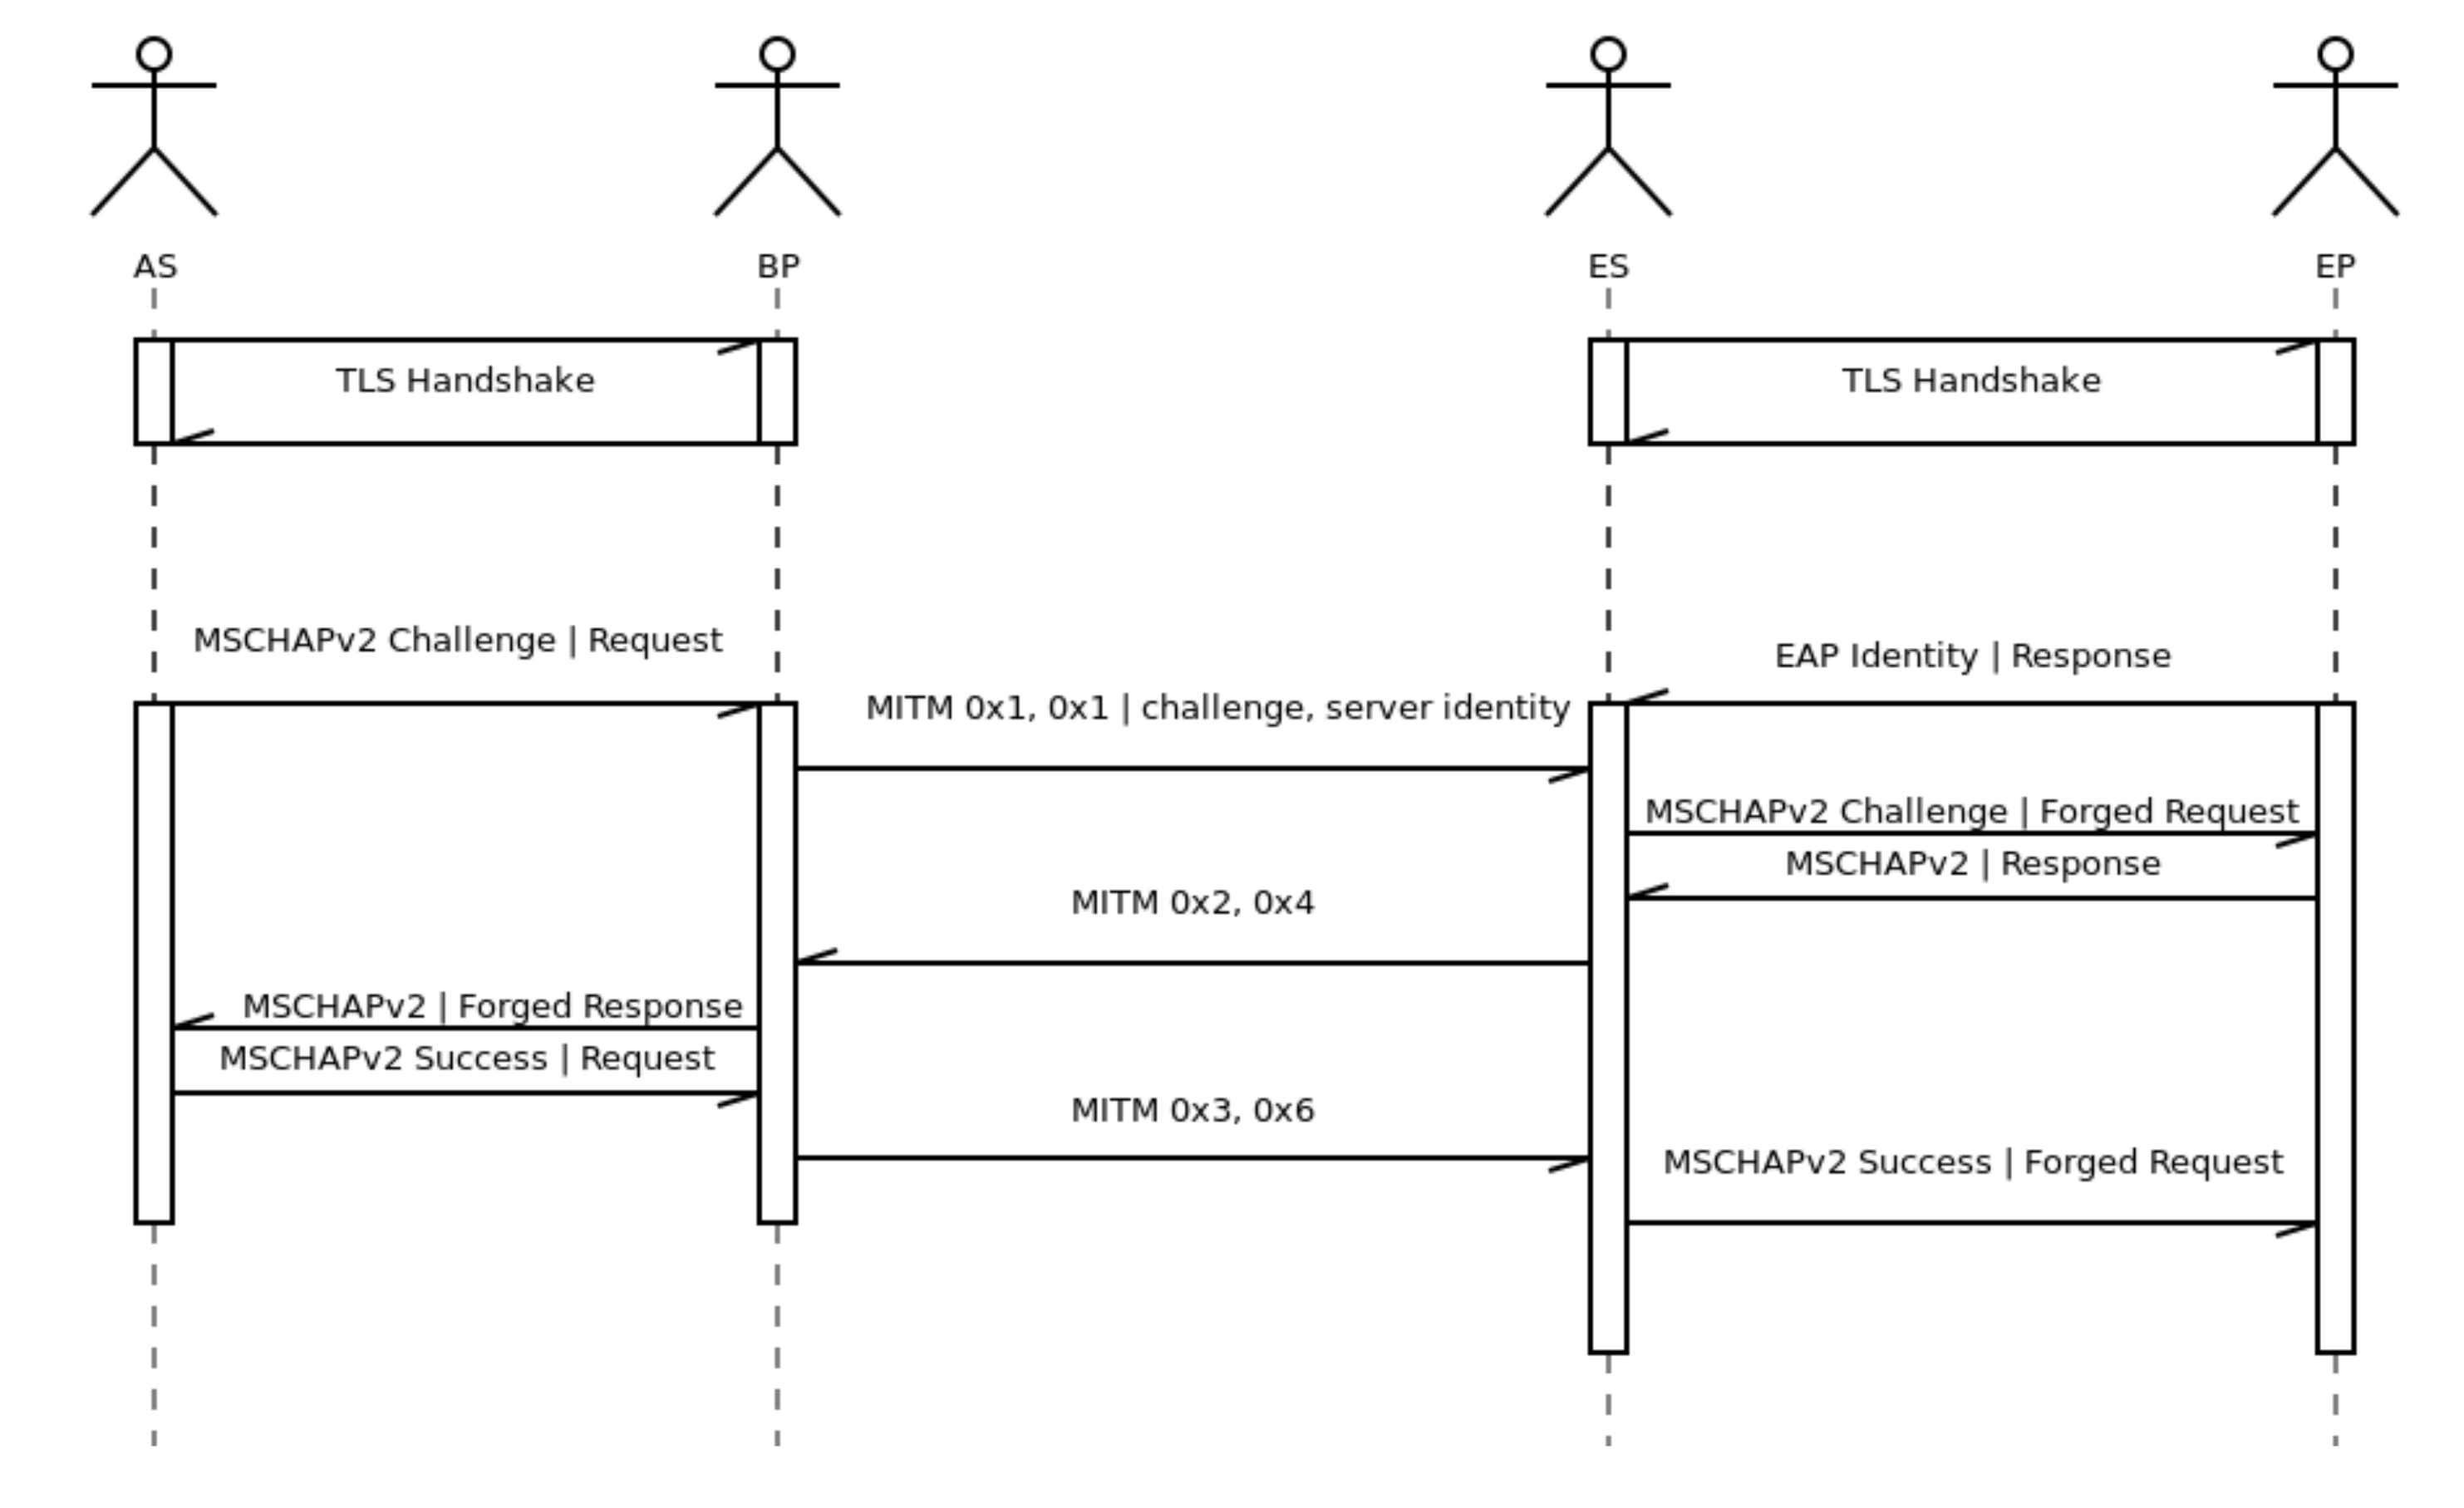
\includegraphics[scale=0.5]{res/clarified-mschapv2-mitm-in-peap.png}
  \caption{Детальная проброска MSCHAPv2}
\end{figure}

\subsection{Анализ кодовой базы}

Для достижения желаемого эффекта нам очень важно разобраться
с конкретной реализацией всех упомянтых сущностей.
К счастью, код отлично соотвествует RFC 4137 \cite{rfc4137},
где определяется архитектура в деталях для этих самых
EAP автоматов.
Там присутствуют оба автомата -- клиентский и серверный.
Для автомата  EAP Сервера был рассмотрен аутентификатор
с автономным функционированием.

В первую очередь, мы протестировали стандартное поведение,
это было о чень важно, так как мы искали когда уязвимость существует
и когда её нет.
Криптобиндинг упомянутый в \cite{tap2002} реализован в современном
автомате действительно:
сессионный ключ создается Pseudio Random Function Plus (PRF+),
он основан на главенствующем секрете  TLS $T$ и ключе второй фазы $S$
полученный в близи окончания внутреннего протокола аутентификации.
Детальный алгоритм досутпен в \cite{josefsson-draft-10}.
Важно добавить, что версия 5 \cite{josefsson-draft-05}
той же спецификации PEAP говорит, что сессионные ключи
базируется лишь на главенствующем секрете $T$.
Как это и было в \cite{tap2002}, из-за чего были проведены исслования
таких схем шифрования.
Интернет поиск говорит, что роутеры Cisco имеют криптобиндинг с 2004,
но эта функциональность опциональна.
В hostap было обнаружено, что TLV Cryptobinding (эта фактическое название
реализации протокола)
всегда инициалзируется сервером,
и включает не только явное связывание,
но и генерацию сессионных ключей на базе $T$ и $S$.
Если криптобиндинг выключен,
поведение соотвествует \cite{josefsson-draft-05} в PEAP протоколе,
то есть уязвимо к MitM атаке,
конечно если только клиент не проверяет сетевой сертификат.

Из кода видно что:
\begin{enumerate}
  \item криптобиндинг присутствует только в PEAPv0,
    PEAPv1 реализация не имеет такой возможности,
    и во многих аспектах тот же PEAPv0.
  \item клиент не может попросить сервер для проведения криптобиндинга,
    он может только отказаться от соединения.
    Это происходит, когда клиентские настройки требуют криптобиндинг,
    но сервер не использует его, либо помечает это опциональным
    в конфигурации hostap.
\end{enumerate}

И так мы выключаем проверку сертификата сервера у Клиента Боба,
то есть не предоставляем никакого сетификата в конфигурации.
Затем для выключения криптобиндинг мы требуем версию PEAP
быть равной 1 на обоих сторонах.
Для небольшого разнообразия, MitM проверяет сертификат сервера,
но трубет PEAPv1.
В добавок, Клиент Евы и Сервер Евы оставлены без какого-либо
пароля пользователя.
Хотя, для некоторого облегчения,
имя пользователя оставлено без изменений
как в исходном примере  eap\_example.
В любом случае, оно моожет быть получено, так как клиент
посылает его личность дважды,
перед TLS Handshake (в соответствии с PEAP),
и внутри TLS туннеля вначале внутреннего протокола аутентификации.
И его личность передаётся в открытом тексте, либо зашифрована
скомпрометированным TLS туннелем.

\subsection{Частные заметки о реализации hostap}

Теперь давайте детально обсудим особенности реализации hostap.

Изначально автомат EAP не позволяет запросам и ответам простаивать.
Но в MitM атаке Клиент и Сервер Евы вынуждены ждать
время от времени, ведь они общаются между собой посредством
MitM автоматов.
Оказывается, что такое поведение было нужно и разработчики hostap
предоставили такой функционал.
С нашей стороны мы используем это достаточно часто,
хотя некоторые правки в коде PEAP были необходимы
для достижения желаемого эффекта.
Возможность простаивания играет важную роль в прерывании
автоматов с их последующем возобновлением.
Обычно, TLS имеет защиту против атак дублированием,
и мы не можем просто повторить сообщение PEAP для автомата Евы,
когда мы получили соответствующие данные,
для продолжения проброса MSCHAPv2.
Но простаивание позволяет это путем функции обратного вызова,
который сохраняет расшифрованные данные от нужного сообщения,
и восстанавливает позже работу EAP метода с тем же параметрами,
сохраненными на предыдущем шаге.
Новый пакет всегда игнорируется, если машины была в состаянии
простаивания на прошлом шаге.
Но он оказывает значительную услугу путем приведения в действие
EAP автомата таким образом, что автомат повторяет практически
те же действия, что и на предыдушем шаге, но теперь
метод может завершиться полноценно и сгенерировать нужное сообщение
или перейти в следующее состояние.
Без этого, результирующий код получилося в разы сложнее.

Автомат означает граф, где состояния (вершины) соединены
посредством переходов (дуг), которые описывают условия и фактические
направления изменения состояния.
Автомат может производить некоторые действия когда он переходит
в состояние или когда происходит соответствующий переход.
В EAP автоматах действия содержятся в состояниях.
В автомате MitM, мы производим действия во время перехода.

На рисунках 4, 5 и 6, 7 представлены Клиент и Сервер EAP,
а также Клиент и Сервер MitM автоматов.

\begin{figure}
  \centering 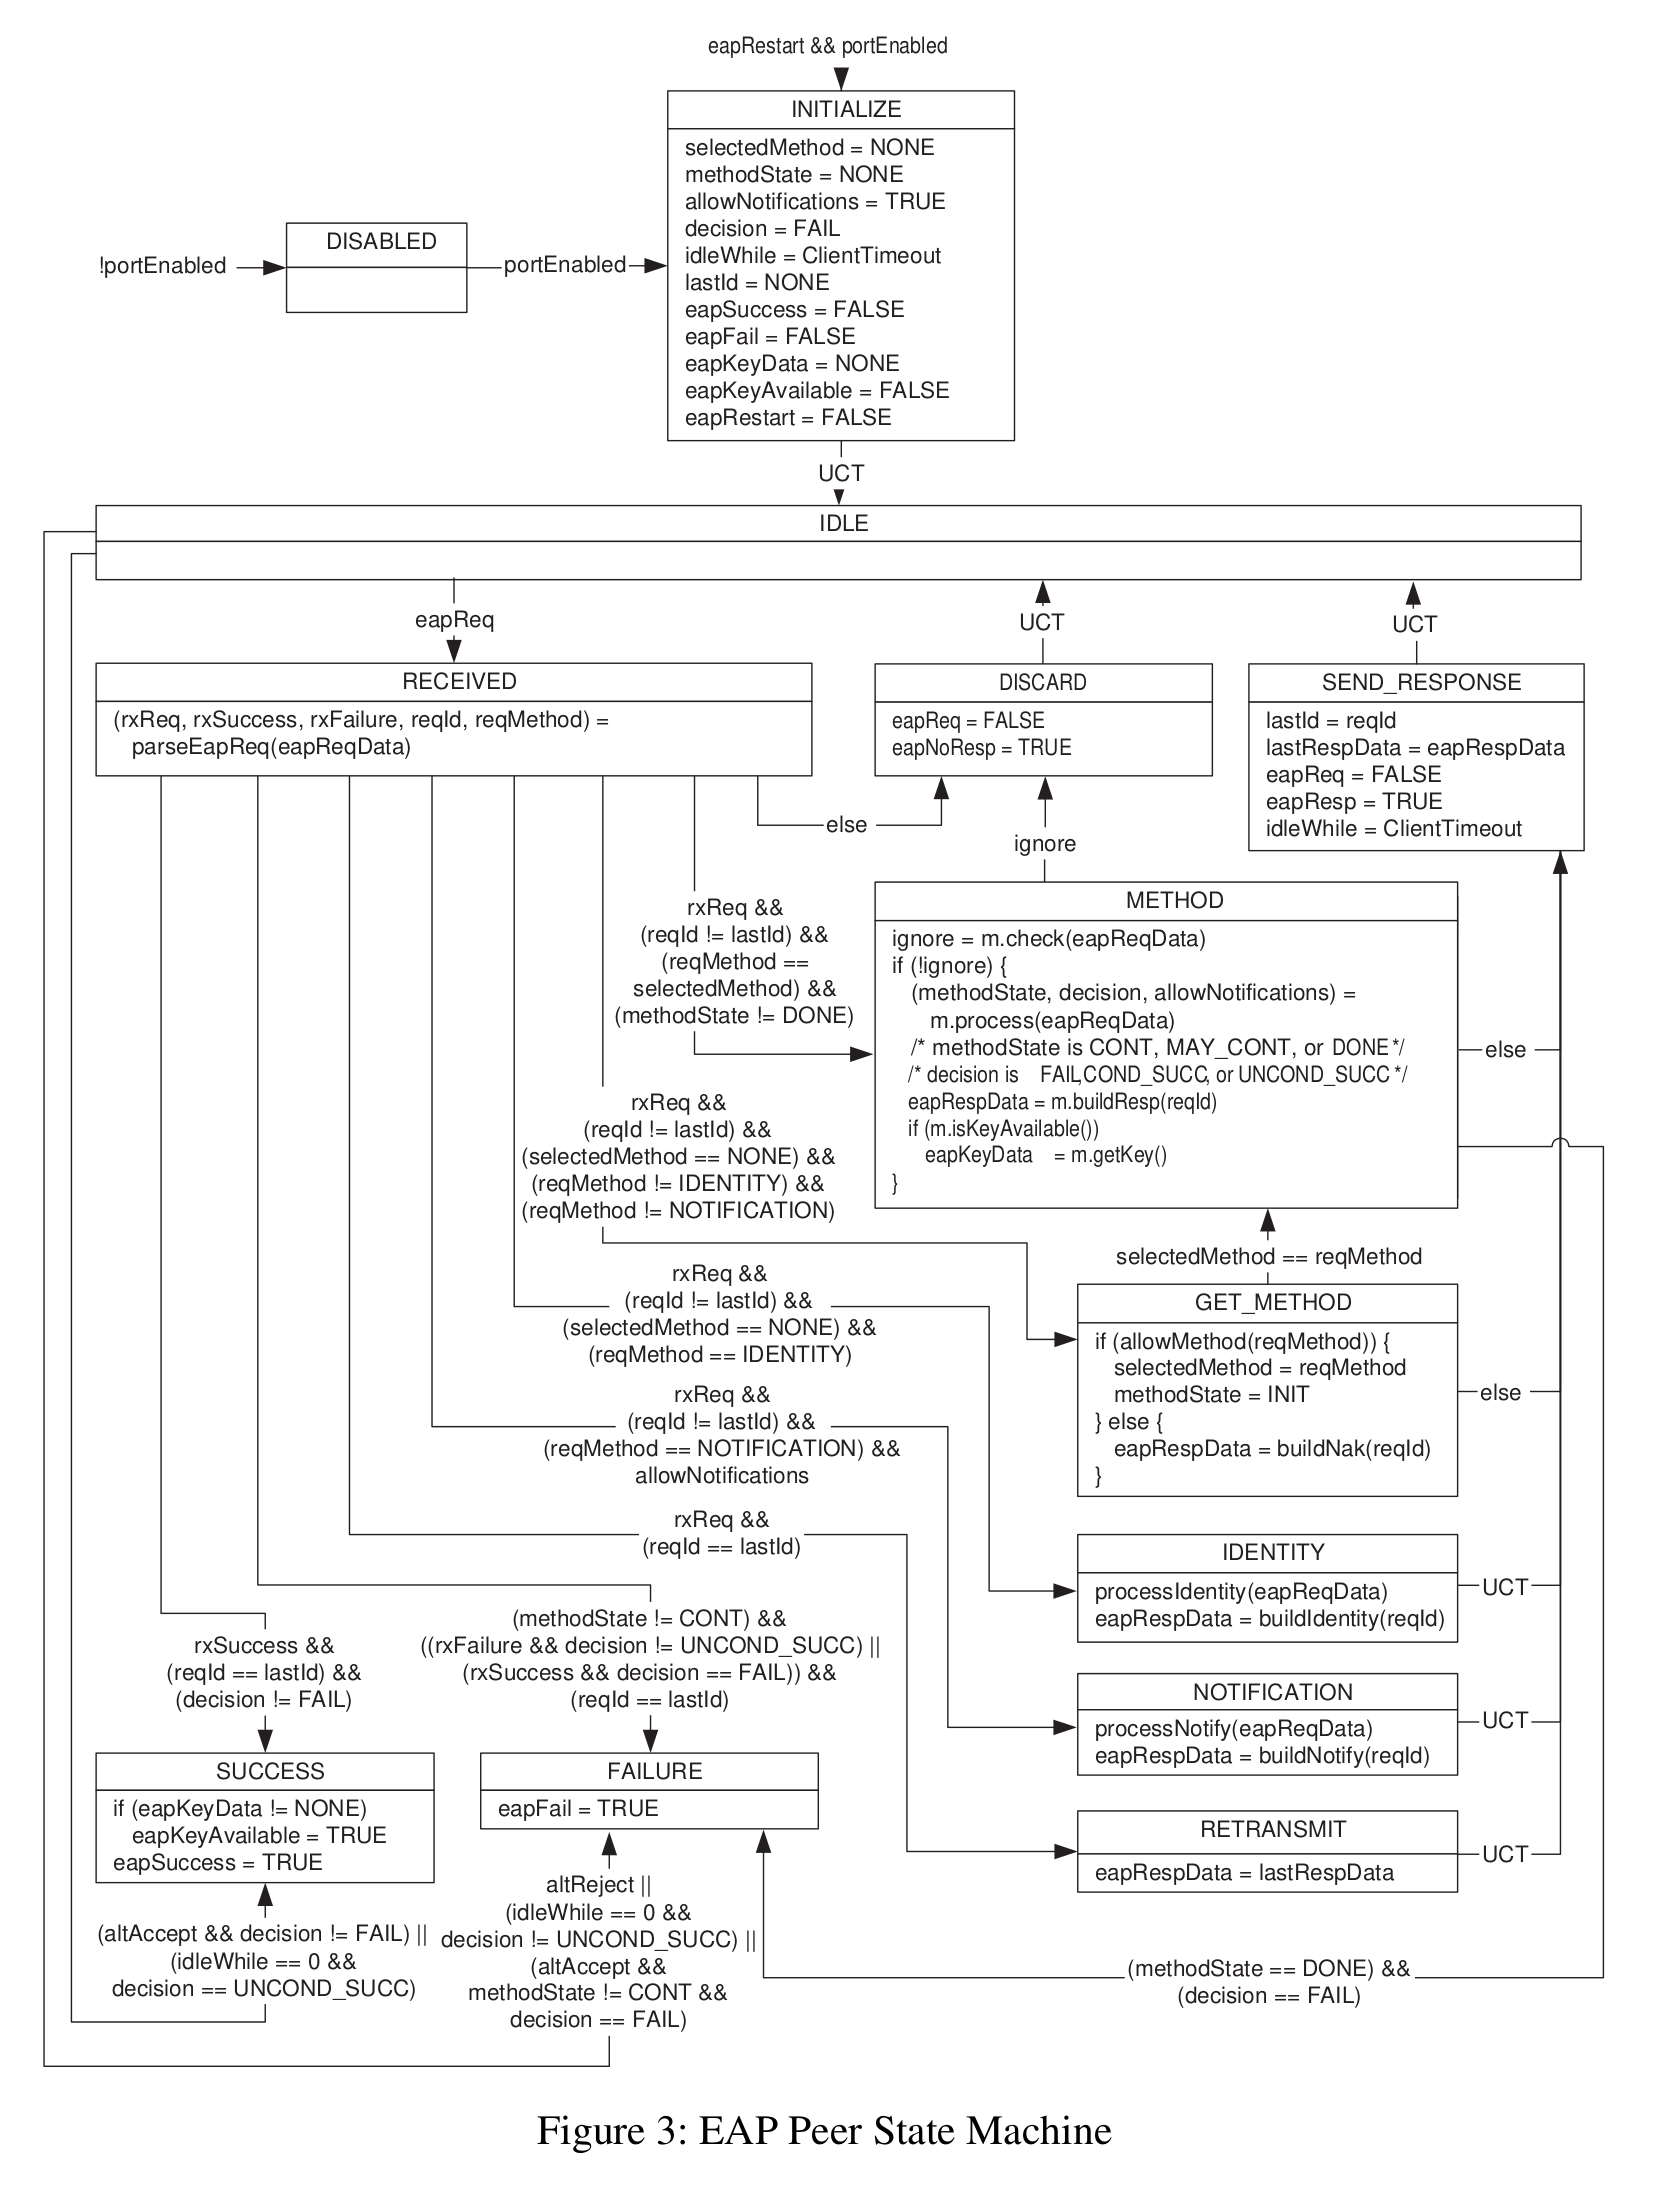
\includegraphics{res/eap-peer-state-machine-rfc4137.png}
  \caption{Автомат EAP Клиента, из RFC4137}
\end{figure}

\begin{figure}
  \centering 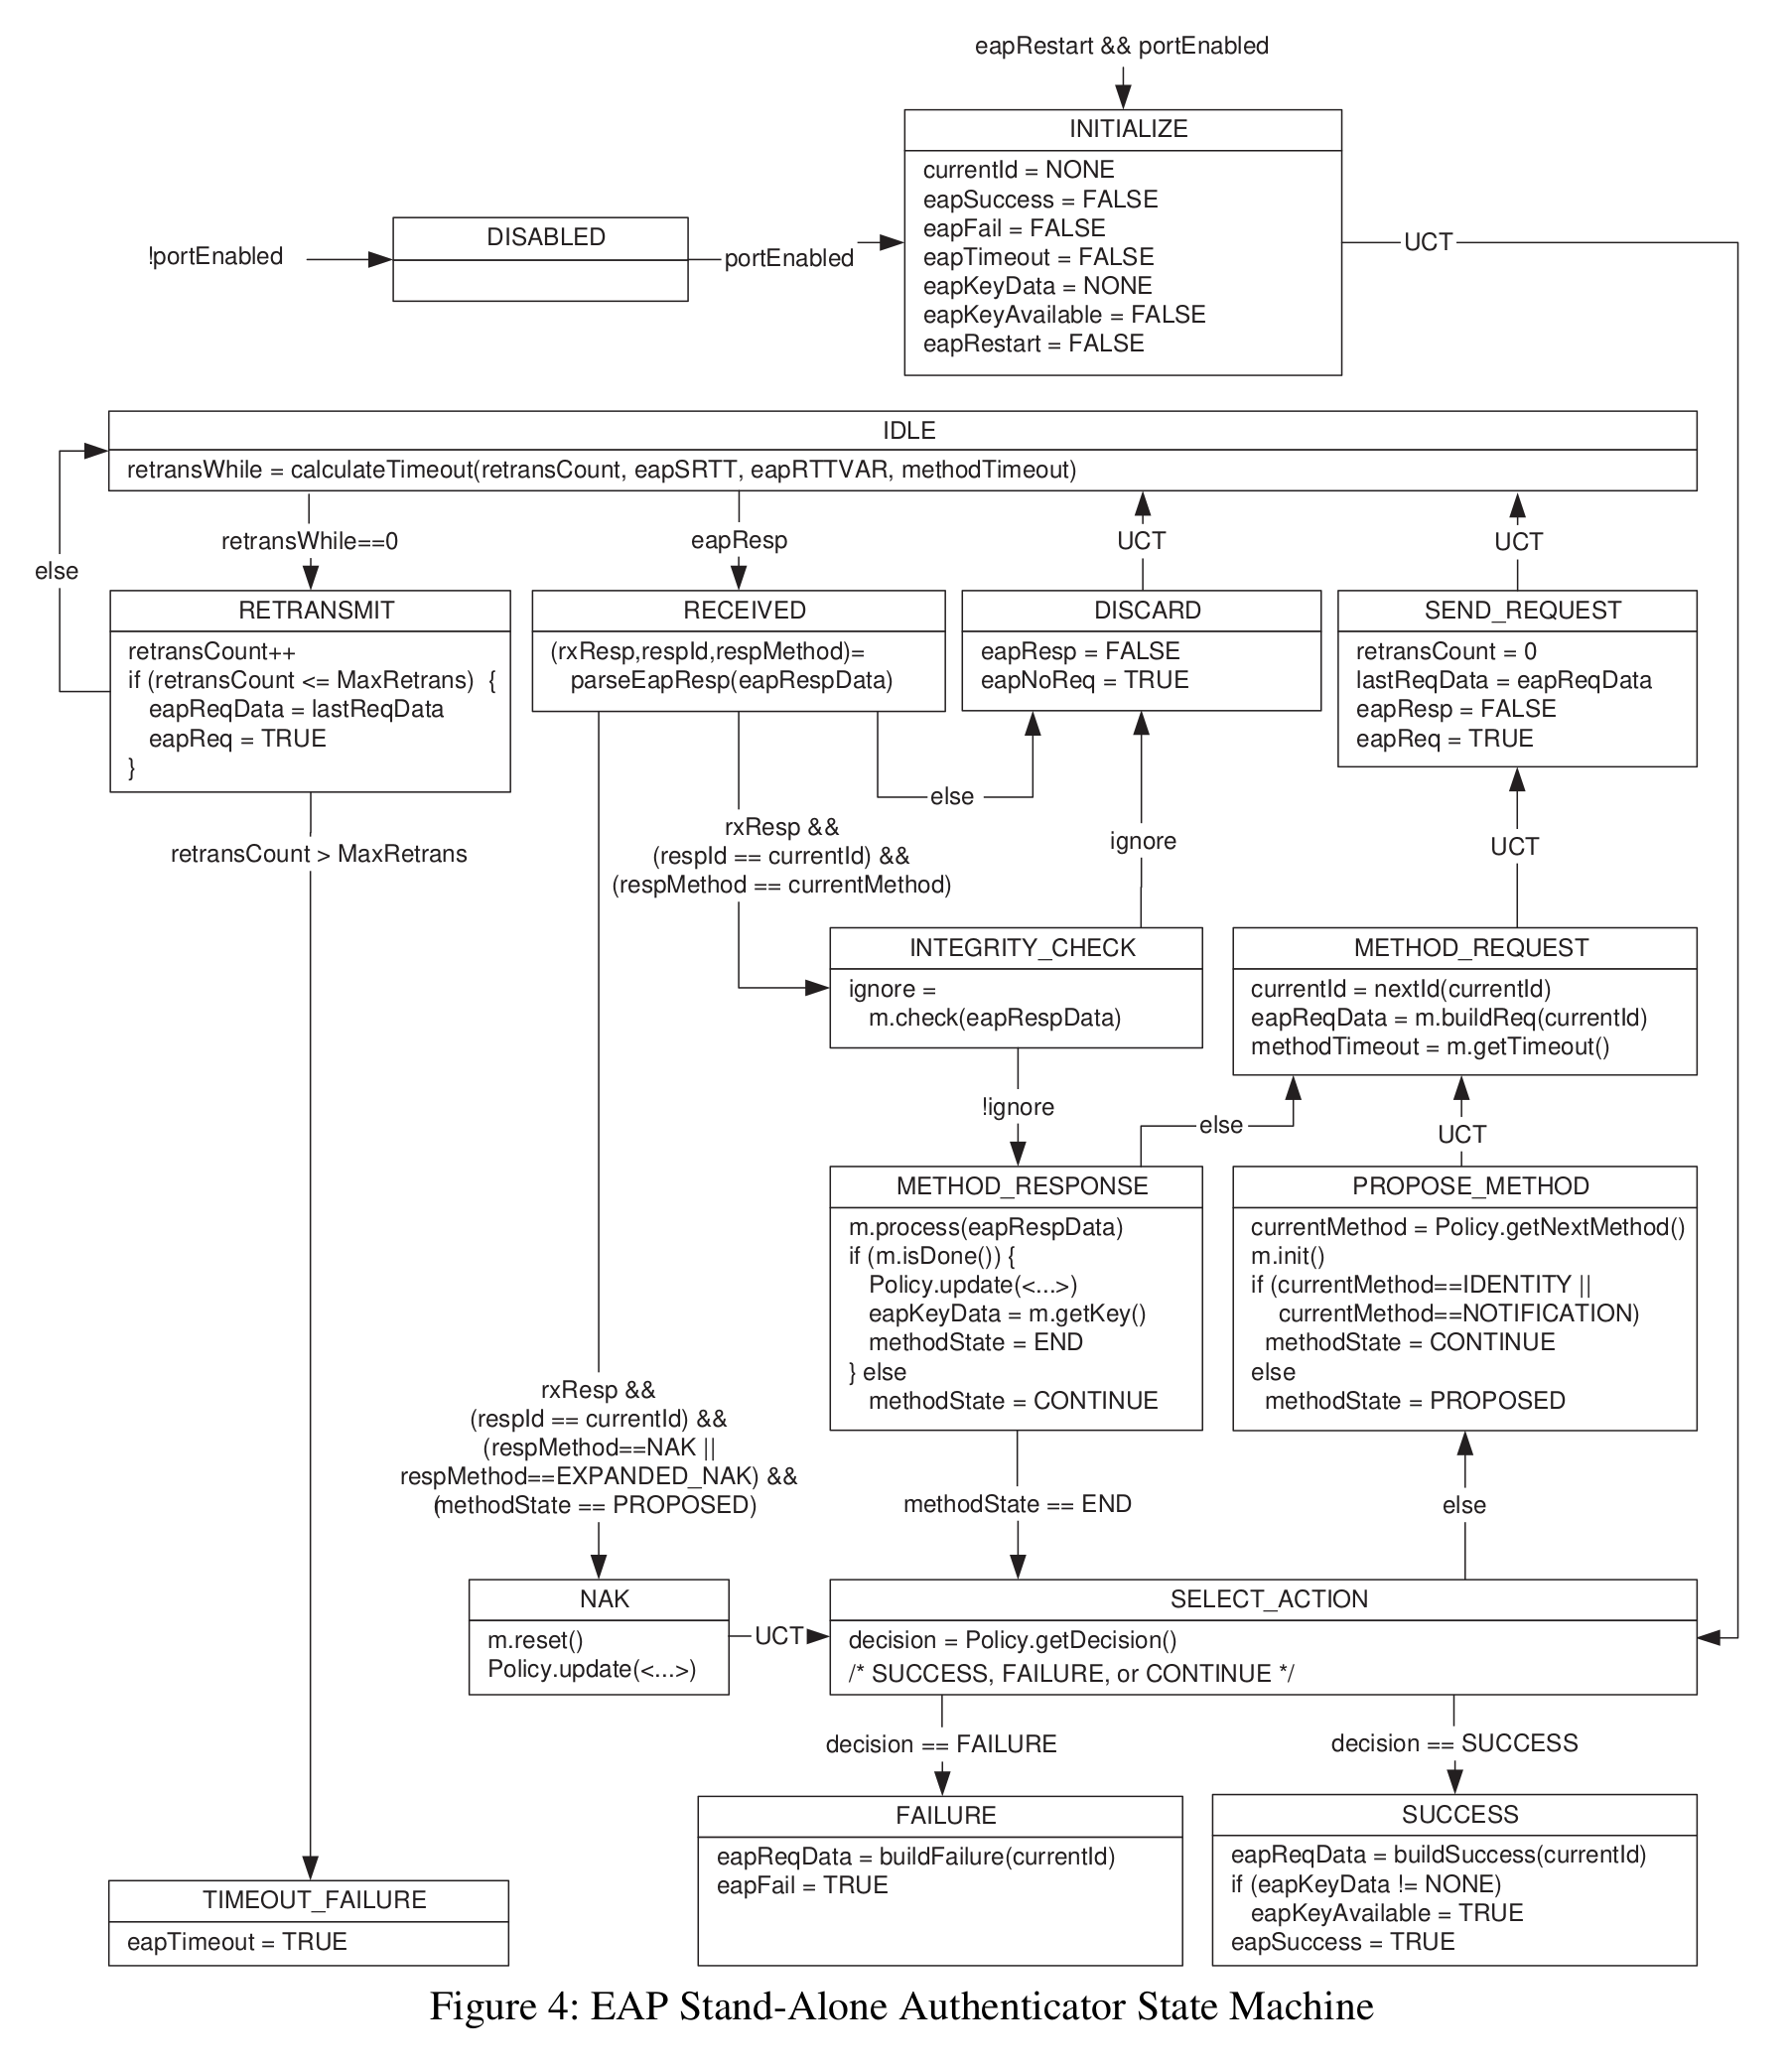
\includegraphics{res/eap-server-state-machine-rfc4137.png}
  \caption{Автомат EAP Сервера, из RFC4137}
\end{figure}

\begin{figure}
  \centering
  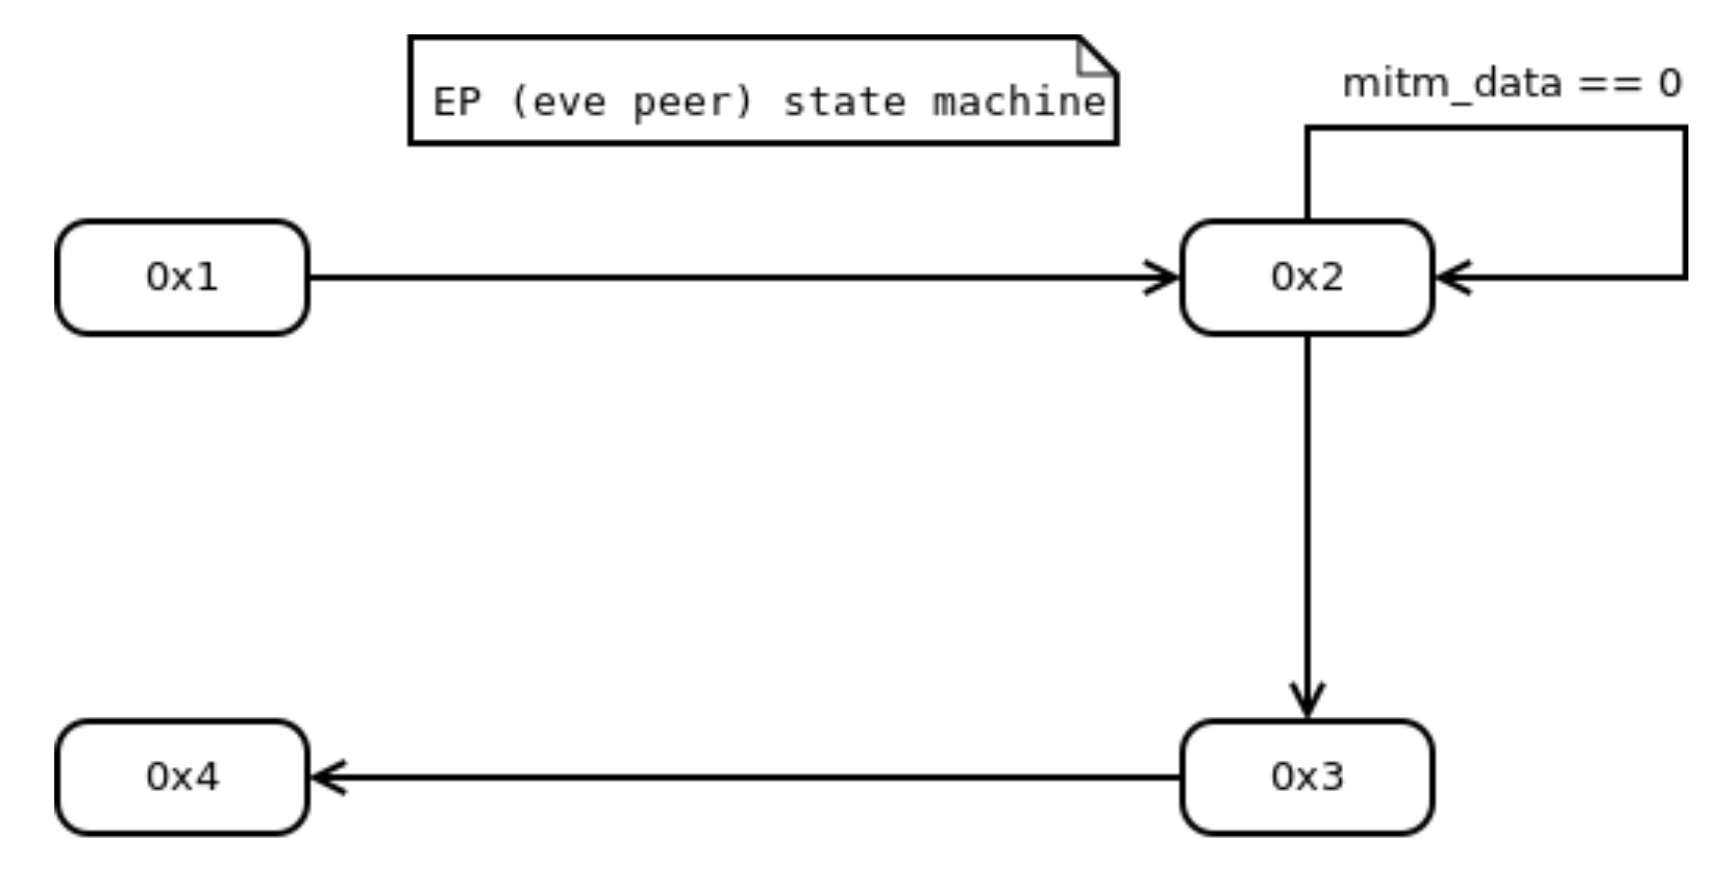
\includegraphics[scale=0.5]
    {res/eve-peer-mitm-state-machine-diagram.png}

  0x1 $\rightarrow$ 0x2
  \begin{enumerate}
    \item Посылка сообщения протокола MITM с MSCHAPv2 Challenge
      Request от AS(Сервера Алисы)
  \end{enumerate}

  0x2 $\rightarrow$ 0x3
  \begin{enumerate}
    \item Получение сообщения протокола MITM с MSCHAPv2 Challenge
      Response от BP (Клиента Боба)
    \item Конструирование поддельного MSCHAPv2 Challenge
      Response используя приобретённый Challenge Response
  \end{enumerate}

  0x3 $\rightarrow$ 0x4
  \begin{enumerate}
    \item Посылка сообщения протокола MITM с MSCHAPv2 Challenge
      Response от BP(Клиента Боба)
    \item Конструирование поддельного MSCHAPv2 Success
      Response без проверки Authenticator Response в Success Request
  \end{enumerate}
  \caption{Автомат Клиента MitM}
\end{figure}

\begin{figure}
  \centering 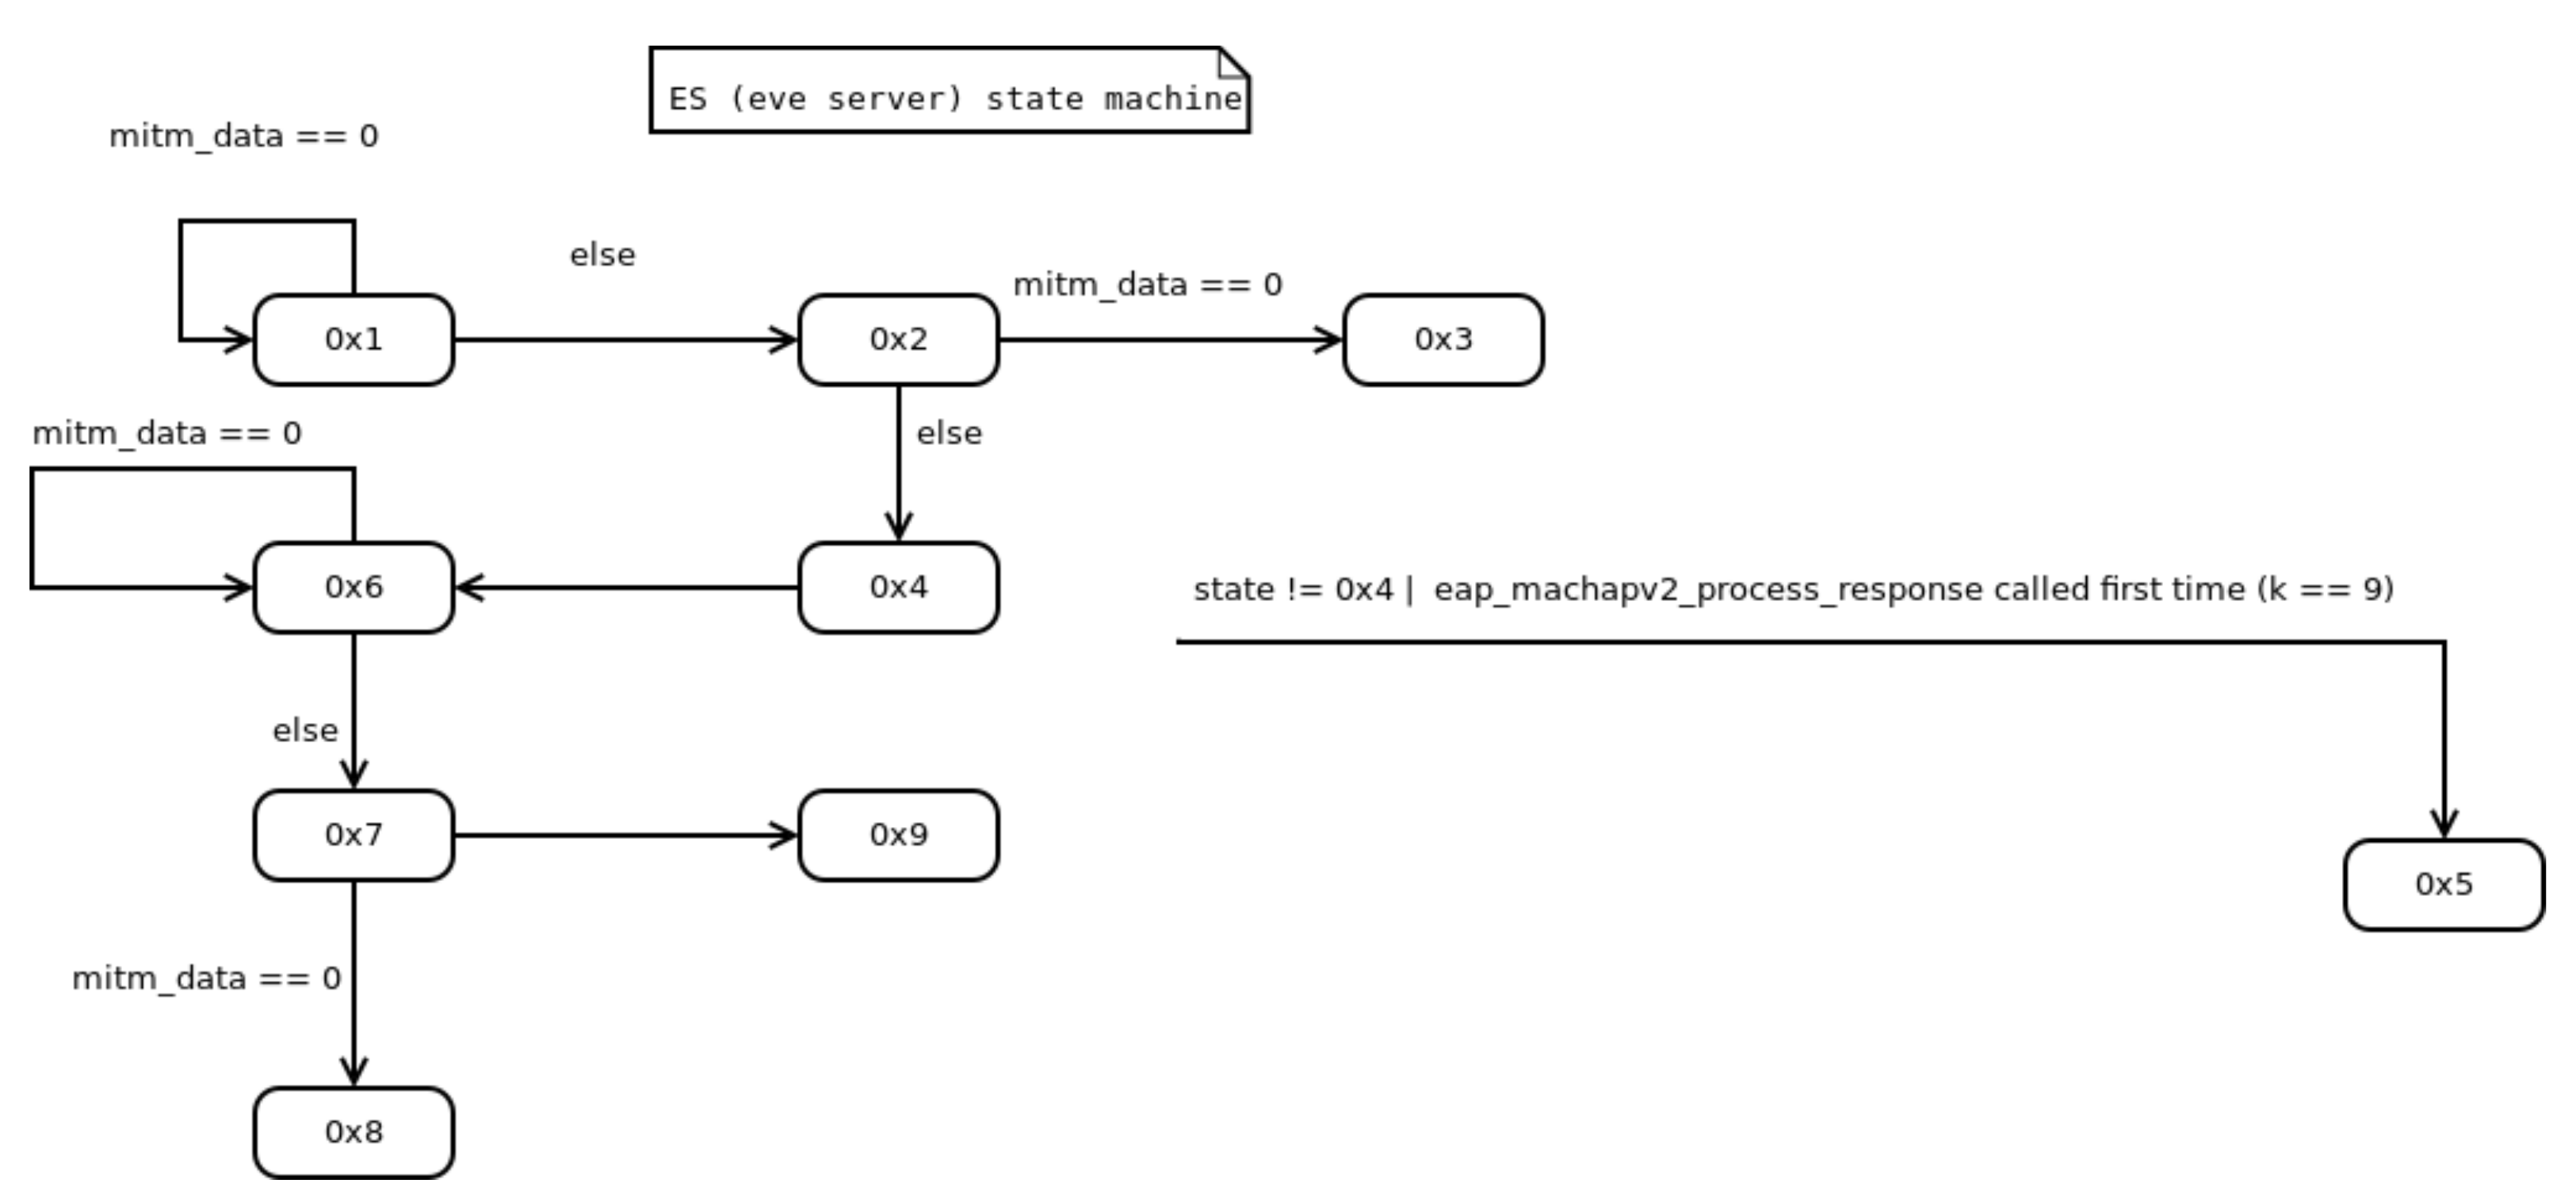
\includegraphics[scale=0.5]
    {res/eve-server-mitm-state-machine-diagram.png}

  0x1 $\rightarrow$ 0x2
  \begin{enumerate}
    \item Получение сообщения MITM протокола: MSCHAPv2 Challenge
      Request от AS (Сервер Алисы)
  \end{enumerate}
  0x2 $\rightarrow$ 0x3, 0x* $\rightarrow$ 0x5, 0x7 $\rightarrow$ 0x8
  \begin{enumerate}
    \item Failure
  \end{enumerate}
  0x2 $\rightarrow$ 0x4
  \begin{enumerate}
    \item Построение поддельного MSCHAPv2 Challenge
      Request используя полученный auth\_challenge и server\_id
  \end{enumerate}
  0x4 $\rightarrow$ 0x6
  \begin{enumerate}
    \item Передача сообщения MITM протокола с MSCHAPv2 Response от BP(Клиент Боба)
  \end{enumerate}
  0x6 $\rightarrow$ 0x7
  \begin{enumerate}
    \item Получение сообщения MITM протокола MSCHAPv2 Success
      Request от AS (Сервер Алисы)
    \item Пропуск проверки Challenge Response,
      state = SUCCESS\_REQ, master\_key\_valid=1
  \end{enumerate}
  0x7 $\rightarrow$ 0x9
  \begin{enumerate}
    \item Построение поддельного MSCHAPv2 Success Request используя полученный Success Request
  \end{enumerate}
  \caption{Автомат Сервера MitM}
\end{figure}

Код примера eap\_example приводит автоматы в действие для совершения шага
один за одним,
и если новое сообщение сгенерировано хотя одной из машин, итерация цикла повторяется.
В реальной жизни, все автоматы будут действовать параллельно,
и на различных устройствах.
Физическое общение является задачей EAPOL автомата,
то есть EAP по LAN.
Автомат отвечает за работу EAP автоматов и доставку
их сообщений.
Общение между парой Клиент Боба и Сервер Евы,
и парой Клиент Евы и Сервер Алисы происходит естественно
так как Клиент Евы вероятнее всего будет экземпляром wpa\_supplicant,
а Серве Евы  -- экземпляром hostapd.
Остальные два автомата не суть важны для атакующего.
Для соединения автоматов MitM, мы вероятнее всего должны воспользоваться
сокетами.
Но следует сново повторить, что мы представляем лишь симуляцию.
В которой все пакеты передаются путём простого копирования буфера с данными внутри
одного процесса.

\cleardoublepage

\section{Отчёт о разработке}

Здесь представлен отчёт о поведении симуляции
после каждого нового коммита, примененного
поверх предыдущего.

%\textbf{commit 242fc738a057}
%
%Peer is authenticated by Server within a TLS 1.2 tunnel,
%with a help of PEAPv0 with MSCHAPv2. By the end of conversation
%TLV Cryptobinding protocol is performed.
%
%\textbf{commit 3d38acc54e62}
%
%EAP behaviour is the same. Commits contains not related changes.
%
%\textbf{commit cf8b14eb9c93}
%
%EAP behaviour is the same. But secret material is revealed in log,
%i.e. TLS master secret, EAP keying material and etc.
%
%\textbf{commit 26d71ce309d3}
%
%EAP behaviour is the same. EAP state machine data was incapsulated
%into instance\_data structure. See commit message for more details.
%
%\textbf{commit c08e56344833}
%
%The EAP behaviour was duplicated. Two pairs of state machines
%communicate between each other -- Bob Peer and Eve Server,
%and Eve Peer and Alice Server.
%
%\textbf{commit 024a2b3685aa}
%
%Bob Peer was configured to skip network certificate verification
%obtained from Eve Server.
%
%\textbf{commit 9a2cd78574c6}
%
%Bob Peer forces PEAPv1, the same actions are taken
%by Alice and Eve Server. It alleviates TLV Cryptobinding
%as well as forces EAP keying material to be derived
%from TLS master secret only.
%
%\textbf{commit bc0150b8dadb}
%
%Eve Peer and Eve Server are delayed for some time.
%To achieve the behaviour pending request and pending response
%functionality of hostap implementation was utilized.
%
%Both Eve Peer and Eve Server are waiting 10 iterations
%processing the very same packets -- MSCHAPv2 Challenge Request
%for Eve Peer,
%and EAP-Identity Response for Eve Server.
%After 10 iterations they proceed with usual behaviour.
%
%\textbf{commit b88c9c348287}
%
%Eve Peer puts MSCHAPv2 Challenge and server\_id into mitm\_data
%buffer and remains in pending state as usual.
%Eve Server waits for a new message,
%after that he continues usual behaviour of EAP-Identity Phase2 method.
%
%So despite of the message transmission,
%Eve's state machines end up as usual after waiting iterations.
%
%Both pairs still communicates independently as in default eap\_example.
%
%\textbf{commit 7964f349cbbe}
%
%Eve Server generate MSCHAPv2 Challenge Request with a challenge
%from Alice Server.
%
%The communication ends up succefully, as Eve Server possesses
%user identity and password.
%
%There is no simulation, except for generating random challenge
%by Alice Server only. And Eve Server takes it, by receiving
%a message from Eve Peer MitM state machine, to generate
%challenge request.
%
%\textbf{commit  764f22d88a12}
%
%EAP behaviour is the same. Commit enables CONFIG\_TESTING\_OPTIONS
%to generate asleap utility commands. Such a behaviour
%resembles the attack from SHMOOCON presentation.
%
%In other words, we can start up a hostapd instance, which
%has the name of a target NAS. And to repeat the attack
%all we need is to enable asleap commands generation.
%
%By the end of communication log will contain proper
%dictionary attack commands for all clients, that
%were trying to authenticate at our server.
%
%\textbf{commit 0ccda46808674}
%
%Eve Server MitM state machine transmits MSCHAPv2 Challenge
%Response obtained from Bob Peer to Eve Peer MitM state machine.
%Eve Server ignores
%all response verification routins as well as MSCHAPv2 master
%key derivation. It will be user later, when replying with a forged
%MSCHAPv2 Success Request.
%
%The simulation is still not correct,
%as by the end of  waiting loop, Eve Server takes user password
%to verify Challenge Response and generate Success Request.
%
%Eve Peer also authenticates correctly, because the only alteration
%is transmission of Challenge Request from Alice Server to Eve Server.
%Eve Peer as well uses the same password as Bob Peer.
%
%\textbf{commit 1a1149e963aca}
%
%Eve Peer sends to Alice Server correct challenge response,
%botained by Eve Peer MitM state machien from Eve Server MitM state machine.
%Alice Server authenticates Eve Peer.
%But Eve Peer fails to accept success requst from Alice Server
%as the default eap\_example behaviour should do.
%Because MSCHAPv2 Peer Challenge is not equal to the one produced by Bob Peer.
%In further commits, Eve Peer will simply ignore this verification
%as the protocol relies on user consciousness only.
%And it is right, since Eve Peer is the attacker,
%and the legitimate client.
%
%For now we may say that the simulation is partially succeeded.
%Since the attacker was authenticated by original server,
%and all we need is to properly finish MSCHAPv2 Sucess Request verification
%and reply with a proper MSCHAPv2 Success Response, that doesn't
%require any special knowledge from Eve Peer.
%
%The only reason to forge MSCHAPv2 Success Request for Bob Peer
%is to make him tunneling his network traffic through MitM node.

\textbf{commit 4a46fa992e7ca}

Клиент Евы захватывает Success Request от Сервера Алисы.
Клиент Евы управляет своей машиной типа человек-по-середине
для пересылки сообщения аналогичной машине Сервера Евы,
которая принимает сообщение и возобновляет работу Автомата EAP
на стороне Сервера Евы.

Следующий шаг Сервера Евы это построение поддельного MSCHAPv2 Success Request,
с помощью такого же, сгенерированного Сервером Алисы и полученного Клиентом Евы.

К текущему моменту, оба Клиенте Евы и Клиент Боба относят MSCHAPv2 Success
Request к неверным. Первый из них не владеет верным секретным материалом,
в то время как другой, Клиент Боба, получиает действительно неверный
запрос.

\textbf{commit 9cebe623049fe}

Сервер Евы применяет полученный MSCHAPv2 Success Request
для генерирования соответствующего MSCHAPv2 Request для Клиента Боба.
Который он благополучно принимает.
Общение между Сервером Евы и Клиентом Боба завершается успешно.
Обе стороны создают один и тот же материал ключа
известный Серверу Евы.

Для завершения симуляции атаки, нам нужно аутентифицировать
Клиент Евы,
потому что сетевой ресурс находиться в власти Сервера Алисы.

\textbf{commit 45d1094c7494c}

Клиент Евы игнорирует проверку MSCHAPv2 Success Request
и отвечает с MSCHAPv2 Success Response.
Общение между Клиентом Евы и Сервером Алисы
завершается успешно. Обе стороны производят
один и тот же материал для создание ключей
основанный только на главенствующем секрете TLS.
С этого момента Сервер Алисы должен принимать
сетевой траффик, и данные будут шифроваться с помощью
ключа известного Клиенту Евы.

В реальной атаке человек-по-середине, Сервер Евы
и Клиент Евы должны начать проброс сообщений между Клиентом Боба
и Сервером Алисы.
Они оснащены всеми необходимыми ключами для компрометирования
туннелей.
Как преимущество атаки,
Ева может слать любые дополнительные сетевые сообщения,
поскольку имеется полностью аутентифицированный и авторизованный
доступ к сети.
В атаке человек-по-середине, главная цель это анализ траффика жертвы.
Данная цель достигнута успешно.

\cleardoublepage

\section{Заключение}
Хочется отметить, что симуляция была успешной
и благодяра хорошей кодовой базе hostap,
не отняла много времени при реализации.
Хотя мы можем только мечтать о её применении в реальной жизни.

\cleardoublepage

\addcontentsline{toc}{section}{\bibname}

\begin{thebibliography}{99}
  \bibitem{tap2002}
    Nokia Research Center,
    Man-in-the-Middle in Tunneled Authentication Protocols,
    11 Ноября 2002 года. \\
    http://eprint.iacr.org/2002/163/
  \bibitem{GMI}
    https://github.com/nartes/hostap-mitm-mschapv2-peapv1
  \bibitem{josefsson-draft-05}
    https://tools.ietf.org/html/draft-josefsson-pppext-eap-tls-eap-05
  \bibitem{josefsson-draft-10}
    https://tools.ietf.org/html/draft-josefsson-pppext-eap-tls-eap-10
  \bibitem{rfc4137}
    https://tools.ietf.org/pdf/rfc4137.pdf
  \bibitem{hostap-w1fi}
    http://w1.fi/
  \bibitem{hostapd-wpe}
    https://github.com/OpenSecurityResearch/hostapd-wpe
  \bibitem{whfs-peap-shmoocon-2008}
    http://www.willhackforsushi.com/presentations/\\
    PEAP\_Shmoocon2008\_Wright\_Antoniewicz.pdf
\end{thebibliography}
\end{document}
